\documentclass[9pt, aspectratio=169]{beamer}

\usetheme{metropolis}
\setbeamertemplate{itemize items}{\faAngleRight}

\metroset{titleformat=smallcaps,block=fill,numbering=counter,progressbar=frametitle,sectionpage=none}
\setbeamersize{text margin left=5mm,text margin right=5mm} 
% \input{embed_video}
\usepackage{fontspec,minted}
\usepackage[scale=1]{ccicons}
\usepackage{metalogo}
\usepackage{xcolor,colortbl}
\usepackage{multicol,multirow,booktabs}
\usepackage{appendixnumberbeamer}
\usepackage{graphicx}
\usepackage{mismath}
\usepackage{bm}
\usepackage{fontawesome5}
\usepackage{csquotes}
\usepackage[backend=biber, natbib, sorting=nyt, doi=true, url=false, url=false, isbn=false, maxbibnames=10]{biblatex}
\addbibresource{../utils/refs.bib}

\usepackage[spanish, es-nodecimaldot]{babel}
\deftranslation[to=spanish]{Definition}{Definición}
\deftranslation[to=spanish]{Theorem}{Teorema}
\deftranslation[to=spanish]{Example}{Ejemplo}

\usepackage{mathtools, mathrsfs}
\usefonttheme{professionalfonts}
\usepackage{textcomp, wasysym}

\setsansfont[BoldFont={Iwona Heavy}, Numbers={Lining, Proportional}]{Iwona Light}
% \setmathsfont(Digits)[Numbers={Lining, Proportional}]{Fira Sans Light}
\setmonofont[Scale=MatchLowercase]{DejaVu Sans Mono}

\setbeamercolor{alerted text}{fg=red,bg=black!2}
\setbeamercolor{progress bar}{fg=red,bg=red!2}
\setbeamertemplate{itemize item}{\faCaretRight}
\setbeamertemplate{itemize subitem}{ \faAngleRight}
\setbeamertemplate{blocks}[shadow=false]
\setbeamercolor{block title}{bg=black!30,fg=red}
\setbeamercolor{block body}{bg=black!20,fg=black}
\setbeamertemplate{theorem begin}
{%
\begin{\inserttheoremblockenv}
{%
\inserttheoremheadfont
%{Teorema:}
\inserttheoremname
\ifx\inserttheoremaddition\@empty\else\ : \inserttheoremaddition\fi%
\inserttheorempunctuation
}%
}
\setbeamertemplate{theorem end}{\end{\inserttheoremblockenv}}
\makeatother


 
\usepackage{gensymb,amssymb}
\usepackage{siunitx}
\DeclareSIUnit{\nada}{\relax}
\usepackage{upquote}
\usepackage{cancel}
\usepackage{algpseudocode}
\algrenewcommand\algorithmicrequire{\textbf{Requiere}}
\algrenewcommand\algorithmicensure{\textbf{Devuelve}}
\setbeamertemplate{blocks}[shadow=false]

\newcommand{\cx}{\column{0.5\textwidth}}
\newcommand{\cw}[1]{\column{#1\textwidth}}

\author{Manuel Carlevaro}
\date{{\tiny Departamento de Ingeniería Mecánica \\
             Grupo de Materiales Granulares - UTN FRLP \\
             manuel.carlevaro@gmail.com }}
\institute{
  \vspace{6em}
  \centering
  {\tiny
  Cálculo Avanzado \enspace • \enspace 2024 \\
    \faLinux \- $\cdot$ \- \fontspec{TeX Gyre Pagella}\XeLaTeX \- $\cdot$ \- \ccbysa }
}

%% Operadores
\DeclareMathOperator{\sen}{sen}
\DeclareMathOperator{\senc}{senc}
\DeclareMathOperator{\sign}{sign}
\newcommand{\T}[1]{\underline{\bm{#1}}}
\DeclareMathOperator{\Tr}{Tr}
\DeclareMathOperator{\rg}{rg}
\DeclareMathOperator{\cond}{cond}

\usepackage{hyperref}
\hypersetup{
    colorlinks,
    citecolor=blue,
    filecolor=black,
    linkcolor=blue,
    urlcolor=blue
}
\urlstyle{same}

%% Códigos
\usepackage{minted}
\newminted[cpp]{cpp}{linenos,fontsize=\footnotesize,frame=lines,numbersep=4pt}
\newmintedfile[cppcode]{cpp}{linenos,fontsize=\footnotesize,frame=lines,numbersep=4pt}
\newcommand{\mic}[1]{\mintinline{C++}{#1}}

\newminted[py]{python}{linenos,fontsize=\footnotesize,frame=lines,numbersep=4pt}
\newminted[pyc]{pycon}{linenos,fontsize=\footnotesize,frame=lines,numbersep=4pt} % Consola de Python
\newminted[ipy3]{ipython3}{linenos,fontsize=\footnotesize,frame=lines,numbersep=4pt} % Consola de iPython3
\newmintedfile[pycode]{python}{linenos,fontsize=\footnotesize,frame=lines,numbersep=4pt}

\newmintedfile[makef]{basemake}{linenos,fontsize=\footnotesize,frame=lines,numbersep=4pt}
\definecolor{bg}{RGB}{22,43,58}
\newminted[shell]{console}{linenos=false,fontsize=\footnotesize,breaklines=true, frame=single} % Linea de comandos
\renewcommand\listingscaption{Código}

\makeatletter
\AtBeginEnvironment{minted}{\dontdofcolorbox}
\def\dontdofcolorbox{\renewcommand\fcolorbox[4][]{##4}}
\makeatother

% uso:
% Ejemplo de uso explícito:
% \begin{py}
% >>> list("abcd")
% ['a', 'b', 'c', 'd']
% \end{py}
% 
% Ahora ejemplo de código en file:
% \pycode{Chapters/intro/code/hola.py}
% 
% También se puede poner un sector del file:
% \pycode[firstline=6, lastline=7]{Chapters/intro/code/hola.py}
% 
% También se puede poner código \textit{inline}: \mip{print('¡Hola mundo!')} y en una sola línea:
% \slp|if __name__ == '__main__')|
% 
% Por último, se puede poner el código en un entorno \textit{float}, esto es, como las tablas y las figuras, con un caption y un label para luego hacer referencias, como por ejemplo al Código \ref{code:hola}.


\usepackage{tikz}
\usetikzlibrary{shapes,shadows,arrows,positioning,matrix,chains,backgrounds,fit}

\tikzset{
    %Define standard arrow tip
    >=stealth',
    %Define style for boxes
    obj/.style={
           rectangle,
           rounded corners,
           draw, very thick,
           text width=10em, fill=green!20,
           minimum height=2em,
           text centered, drop shadow},
    proc/.style={
	    rectangle, rounded corners,
	    draw,fill=red!50,very thick,
	    text width=8em,minimum height=2em,
	    text centered, drop shadow},
    % Define arrow style
    pil/.style={
           ->,
           thick,
           shorten <=2pt,
           shorten >=2pt,}
}

\setbeamertemplate{bibliography item}{%
  \ifboolexpr{ test {\ifentrytype{book}} or test {\ifentrytype{mvbook}}
    or test {\ifentrytype{collection}} or test {\ifentrytype{mvcollection}}
    or test {\ifentrytype{reference}} or test {\ifentrytype{mvreference}} }
    {\setbeamertemplate{bibliography item}{\faBook}}
    {\ifentrytype{online}
            {\setbeamertemplate{bibliography item}{\faGlobe}}
   {\setbeamertemplate{bibliography item}{\faFileText}}}%
  \usebeamertemplate{bibliography item}}

\defbibenvironment{bibliography}
  {\list{}
     {\settowidth{\labelwidth}{\usebeamertemplate{bibliography item}}%
      \setlength{\leftmargin}{\labelwidth}%
      \setlength{\labelsep}{\biblabelsep}%
      \addtolength{\leftmargin}{\labelsep}%
      \setlength{\itemsep}{\bibitemsep}%
      \setlength{\parsep}{\bibparsep}}}
  {\endlist}
  {\item}
\newcommand{\bcite}[1]{\citeauthor{#1}, \citetitle{#1} (\citeyear{#1})}


\title{Cálculo de raíces de ecuaciones de una variable}
\subtitle{}

%%%%
% Bibliografía
% Epperson - An Introduction to Numerical Method and Analysis - Cap. 3 (c/ejercicios)
% Jaan Kiusalaas - Numerical Methods in Engineering with Python - Cap. 4 **
% Brent - Advanced Mathematics for Engineering Students - Cap 9.1 (Punto fijo)
% Kreyszig - Advanced Engineering Mathematics - Cap 19
% Alex Gezerlis - Numerical Methods in Physics with Python - Cap 5 *
% Salgado - Classical Numerical Analysis - Cap. 15
%%%%

\begin{document}
\maketitle

\section{Introducción}

\begin{frame}
\begin{columns}[t]
\cx
\textbf{Problema:}

\begin{equation*}
    \begin{split}
        f(x) &= 0 \\
        f(x) &= g(x) \implies h(x) = f(x) - g(x) = 0
    \end{split} 
\end{equation*}

\begin{theorem}[Valores intermedios]
Sea $f: [a, b] \rightarrow \mathbb{R}$ una función \textbf{continua} en $[a, b]$ tal que $f(a) < f(b)$. Entonces: $\forall u \in (f(a), f(b))$ existe $c \in [a, b]$ tal que $f(c) = u$.
\end{theorem}
\pause

\textbf{Estrategia general:} %% Salgado
\begin{itemize}
    \item Mostrar que existe al menos una solución ($x^*$)
    \item Aislar una raíz: $D \subset \mathbb{R}$, $x^* \in D$ y $f(x) \neq 0 \; \forall x \in D \setminus \{ x^* \}$
    \item Iterar
\end{itemize}
\pause

\cx
\textbf{Métodos:}  %% Wikipedia https://en.wikipedia.org/wiki/Root-finding_algorithms
\begin{itemize}
    \item \textit{Bracketing} (cerrados)
        \begin{itemize}
            \item \alert{Bisección}
        \item Posición falsa (\textit{regula falsi})
        \item ITP
        \end{itemize}
    \item Interpolación
        \begin{itemize}
        \item Secante
        \item Muller
        \end{itemize}
    \item Iterativos (abiertos)
        \begin{itemize}
            \item \alert{Punto fijo}
            \item \alert{Newton-Raphson}
            \item Secante
        \item Broyden
        \end{itemize}
    \item Combinación de cerrados y abiertos 
        \begin{itemize}
            \item {\color{blue} Brent}
        \item Ridders
        \end{itemize}
\end{itemize}
\end{columns}
\end{frame}

\section{Método de bisección}

\begin{frame}{Método de bisección}
\begin{columns}[c]
\cx
\begin{overprint}
    \onslide<1> 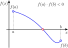
\includegraphics{figs/bisec-01.pdf}
    \onslide<2> \includegraphics{figs/bisec-02.pdf}
    \onslide<3> 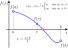
\includegraphics{figs/bisec-03.pdf}
    \onslide<4> 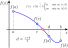
\includegraphics{figs/bisec-04.pdf}
    \onslide<5-> \includegraphics{figs/bisec-05.pdf}
\end{overprint} 
\cx
\begin{overprint}
    \onslide<6> { \begin{theorem}[ Convergencia y error ] % Epperson pg 92
            Sea $[a, b]$ el intervalo inicial, donde $f(a)\cdot f(b) < 0$. Defina una raíz aproximada como 
            \[ x_n = \frac{a_{n-1} + b_{n-1}}{2} \] 
Entonces existe una raíz $x^*$ tal que
 \[ |x^* - x_n| \leq \frac{b-a}{2^n} \]
 Además, para obtener una precisión de $|x^* - x_n| \leq \epsilon$ es necesario iterar $n$ veces con 
 \[ n \geq \frac{\log(b - a) - \log \epsilon}{\log 2} \]
    \end{theorem} }
\end{overprint}

\end{columns}
\end{frame}

\begin{frame}
\begin{columns}[t]
\cw{0.45}
\textbf{Código}

\pycode[firstline=1, lastline=19]{./code/biseccion.py}

\cw{0.45}
\pycode[firstline=20]{./code/biseccion.py}
\end{columns}
\end{frame}

\begin{frame}[fragile]
\begin{columns}[t]
\cw{0.45}
\begin{center}
\includegraphics[scale=0.35]{figs/bisec-ej-01.pdf}
\end{center}

\begin{shell}
$ ./biseccion.py
La raiz de f(x) = 0 es 0.7346035079099238
\end{shell}
\pause

\cw{0.45}
\textbf{SciPy: optimize}

\pycode{./code/scipy-biseccion.py}

\begin{shell}
$ ./scipy-biseccion.py 
La raiz de f(x) = 0 es 0.7346035077880515
\end{shell}

\end{columns}
\end{frame}

\section{Punto fijo}

\begin{frame}{Punto fijo}
    \vspace{1em}
\begin{columns}
\cw{0.45}
$p$ es un \textbf{punto fijo} de $g$ si $g(p) = p$.

Si $g$ tiene un punto fijo en $p$, entonces:
\[ f(x) = x - g(x) \]
tiene un cero en $p$.

\textbf{Ejemplo:} $g(x) = x^2 - 2 \rightarrow p = \{-1, 2\}$.

\begin{center}
    \includegraphics[scale=0.35]{figs/pfijo-ej-01.pdf}
\end{center}
\pause

\cw{0.55}
\begin{theorem}[Existencia y unicidad] % Burden - Faires - Análisis Numérico pg 55
\begin{enumerate}[ i) ]
    \item Si $g \in \mathcal{C}[a, b]$ y $g(x) \in [a, b] \, \forall x \in [a, b]$, entonces $g$ tiene por lo menos un punto fijo en $[a, b]$. 
    \item Si, además, $g'(x)$ existe en $[a, b]$ y hay una constante positiva $k < 1$ con 
        \[ |g'(x)| \leq k, \; \forall x \in [a, b] \]
        entonces existe exactamente un punto fijo en $[a, b]$.
\end{enumerate}
\end{theorem}

\textbf{Iteración de punto fijo:}

\begin{itemize}
    \item Aproximación inicial $p_0$
    \item $\{p_n \}_{n = 0}^{\infty}$ con $p_n = g(p_{n-1}), \; n \geq 1$
    \item Si la sucesión converge a $p$ y $g$ es continua:
        \[ p = \lim_{n \rightarrow \infty} p_n = \lim_{n \rightarrow \infty} g(p_{n-1}) = g \left( \lim_{n \rightarrow \infty} p_{n-1} \right) = g(p) \]
\end{itemize}
\end{columns}
\end{frame}

\begin{frame}[fragile]
    \begin{columns}[t]
\cw{0.45}
\textbf{Código}
\pycode[lastline=21]{code/punto-fijo.py}

\cw{0.45}
\pycode[firstline=23]{code/punto-fijo.py}

\begin{shell}
> ./pfijo.py 
  0 0.2610000000000000 0.1610000000000000
  1 0.5593491000000000 0.2983491000000000
  2 0.7147852845546510 0.1554361845546509
... ... 
 94 0.6551757611798358 0.0000070667498989
 95 0.6551694011125498 -0.0000063600672859
La raiz de g(x) = 0 es 0.6551694011125498
\end{shell}
\end{columns}
\end{frame}

\begin{frame}{Gráfico \textit{coweb}}
\begin{columns}
\cw{0.3}
\begin{center}
    \includegraphics[scale=0.35]{figs/coweb-01.pdf}
    \begin{align*}
        r &= 2.9 \\
    p = g(p) &= \frac{19}{29} \\
    g'(p) &= -\frac{9}{10}
    \end{align*}
\end{center} \pause

\cw{0.3}
\begin{center}
    \includegraphics[scale=0.35]{figs/coweb-02.pdf}
    \begin{align*}
        r &= 3.1 \\
    p = g(p) &= \frac{21}{31} \\
    g'(p) &= -\frac{11}{10}
    \end{align*}
\end{center} \pause

\cw{0.3}
\begin{center}
    \includegraphics[scale=0.35]{figs/coweb-03.pdf}
    \begin{align*}
        r &= 4.0 \\
    p = g(p) &= \frac{3}{4} \\
    g'(p) &= -2
    \end{align*}
\end{center}
\end{columns}
\end{frame}

\section{Método de Newton-Raphson}

\begin{frame}{Método de Newton-Raphson}
\begin{columns}[c]
\cx
\begin{overprint}
    \onslide<1> \includegraphics{figs/newton-01.pdf}
    \onslide<2-> 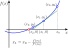
\includegraphics{figs/newton-02.pdf}
\end{overprint} 

\cx
\[ \frac{y - y_0}{x - x_0} = f'(x_0) \Rightarrow  y = f(x_0) + f'(x_0) (x - x_0) \]

Haciendo $y = 0$:
\[x = x_0 - \frac{f(x_0)}{f'(x_0)} \mapsto  x_{n+1} = x_{n} - \frac{f(x_n)}{f'(x_n)}\]
\pause

\begin{overprint}
\onslide<3> {
Serie de Taylor ($x_n \approx x*$):
\[f(x) = f(x_n) + (x - x_n) f'(x_n) + \frac{1}{2} (x - x_n)^2 f''(\xi) \]
$\xi_n \in (x, x_n)$ Hacemos $f(x) = 0$:
\[ x = x_n - \frac{f(x_n)}{f'(x_n)} - \frac{1}{2} (x - x_n)^2 \frac{f''(\xi_n)}{f'(x_n)} \]
\[ \mapsto x_{n+1} = x_n - \frac{f(x_n)}{f'(x_n)'} \]
}
\end{overprint}
\end{columns}
\end{frame}

\begin{frame}[fragile]
    \begin{columns}[t]
\cw{0.45}
\textbf{Código:}

\pycode[lastline=22]{./code/newton-raphson.py}

\cw{0.45}
\pycode[firstline=24]{./code/newton-raphson.py}

\begin{shell}
$ ./newton-raphson.py 
La raiz de f(x) = 0 es 0.7346035077893033.
Iteraciones: 4
La raiz 2 de f(x) = 0 es 0.7346035077893033.
Diferencia: 0.0
\end{shell}
\end{columns}
\end{frame}

\begin{frame}
    \begin{columns}[t]
\cx
\textbf{Convergencia:}
Serie de Taylor alrededor de $\alpha$, ($f(\alpha) = 0$):
\begin{equation} f(\alpha) = f(x_n) + f'(x_n) (\alpha - x_n) + R_1 \end{equation}
Forma de Lagrange de $R_1$:
\begin{equation*}R_1 = \frac{1}{2!} f''(\xi_n) (\alpha- \x_n)^2 \end{equation*}
donde $\xi_n$ está entre $\alpha$ y $x_n$. Como $f(\alpha) = 0$:
\begin{equation}
    0 = f(x_n) + f'(x_n) (\alpha - x_n) + \frac{1}{2!} f''(\xi_n) (\alpha- \x_n)^2
\end{equation}
Dividiendo (2) por $f'(x_n)$ y reacomodando:
\begin{equation}
    \frac{f(x_n)}{f'(x_n)} + (\alpha - x_n) = -\frac{f''(\xi_n')}{2 f'(x_n)} (\alpha - x_n)^2
\end{equation}

\begin{equation}
    \text{NR: }\quad    x_{n+1} = x_n -\frac{f(x_n)}{f'(x_n)}
\end{equation}
\cx
resulta:
\[ \underbrace{\alpha - x_{n+1}}_{\epsilon_{n + 1}} = -\frac{f''\xi_n)}{2 f'(x_n)} (\underbrace{\alpha - x_n}_{\epsilon_n})^2 \]
\begin{equation}
    \left| \epsilon_{n + 1} \right| = \frac{|f''(x_n)|}{2|f'(x_n)|} \cdot \epsilon_n^2
\end{equation}
Convergencia al menos \textbf{cuadrática} si:
\begin{itemize}
    \item $f'(x) \neq 0, \; \forall x \in I \equiv [\alpha - |\epsilon_0|, \alpha + |\epsilon_0|]$
    \item $f''(x) \in \mathcal{C}, \; \forall x \in I$
    \item $M|\epsilon_0| < 1$ con 
        \[ M = \frac{1}{2} \left( \sup_{x \in I} |f''(x)| \right) \left( \sup_{x \in I} \frac{1}{|f'(x)|} \right) \]
\end{itemize}

\[ \boxed{ |\epsilon_{n + 1}| \leq M \cdot \epsilon_n^2 } \]


\end{columns}
\end{frame}

\begin{frame}[fragile]
\begin{columns}[t]
\cx
\textbf{Problemas:}
\begin{itemize}
\item Raíz doble:
\begin{center}
    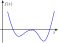
\includegraphics[scale=0.5]{figs/problemas-01.pdf}
\end{center}

\item Divergencia:
\begin{center}
    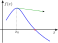
\includegraphics[scale=0.5]{figs/problemas-02.pdf}
    \includegraphics[scale=0.5]{figs/problemas-03.pdf}
\end{center}
\end{itemize}
\pause

\cx
\textbf{Scipy.optimize}

\pycode{./code/root_scalar.py}
\begin{shell}
$ ./root_scalar.py 
Método: bisect , raiz = 0.7346035077910437
Método: newton , raiz = 0.7346035077893033
Método: brentq , raiz = 0.7346035077893016
Método: toms748, raiz = 0.7346035077893033
\end{shell}
\end{columns}
\end{frame}

\section*{Bibliografía}
\begin{frame}[allowframebreaks]{Lecturas recomendadas}
\begin{itemize}
    \item \fullcite{burden2017}. Capítulo 2.
    \item \fullcite{epperson2013}. Capítulo 3.
    \item \fullcite{kiusalaas2005}. Capítulo 4.
 \item \fullcite{kreyszig2011}. Capítulo 19.
\end{itemize}
\end{frame}

\end{document}

